\documentclass{report}
\usepackage{ctex}
\usepackage{graphicx}
\usepackage{amsmath}
\title{表面张力系数的测量}
\author{王启骅 PB20020580}
\begin{document}
	\maketitle
	\section{实验目的}
	用焦利氏秤法测量水和洗洁精溶液的表面张力系数,并通过测量不同浓度的洗洁精溶液的表面张力系数来探究洗洁精溶液表面张力系数和浓度的关系。
	\section{实验原理}
金属丝框缓慢拉出水面的过程中,金属丝框下面将带起一水膜,当水膜刚被拉断时,诸力的平衡条件是$ F=mg+2F' $\quad$ F'=\sigma l $得$ \sigma=\dfrac{F-mg}{2l} $\\
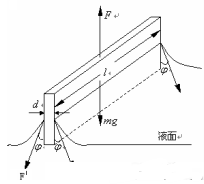
\includegraphics[scale=1]{1}\\
图1:表面张力系数测量原理图
	
	\section{实验仪器}
焦利氏秤、钢板尺、烧杯、砝码。
	\section{实验数据}
\begin{flushleft}
	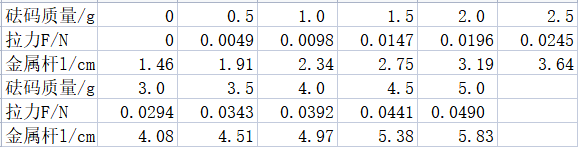
\includegraphics[scale=1]{2}\\
	表1:弹簧劲度系数测量数据表\\
	自来水测量金属杆初读数:$ l_0=1.77cm $\\
	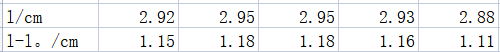
\includegraphics{3}\\
	表2:水表面张力系数测量数据\\
	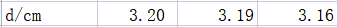
\includegraphics{4}\\
	表3:金属圈直径测量数据表\\
	洗洁精溶液测量金属杆初读数:$ l_0=1.60cm $\\
	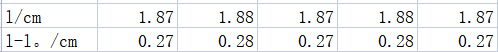
\includegraphics{5}\\
	表4:洗洁精溶液表面张力系数测量数据\\
	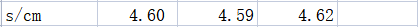
\includegraphics{6}\\
	表5:金属丝两脚距离测量数据表\\
	自配溶液测量金属杆初读数:$ l_0=1.60cm $\\
	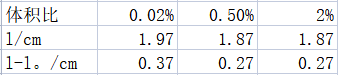
\includegraphics{7}\\
	表6:自配溶液表面张力系数测量数据
\end{flushleft}
	
	\section{数据处理与误差分析}
弹簧劲度系数的测量:对弹簧所受拉力和金属杆读数进行线性拟合\\
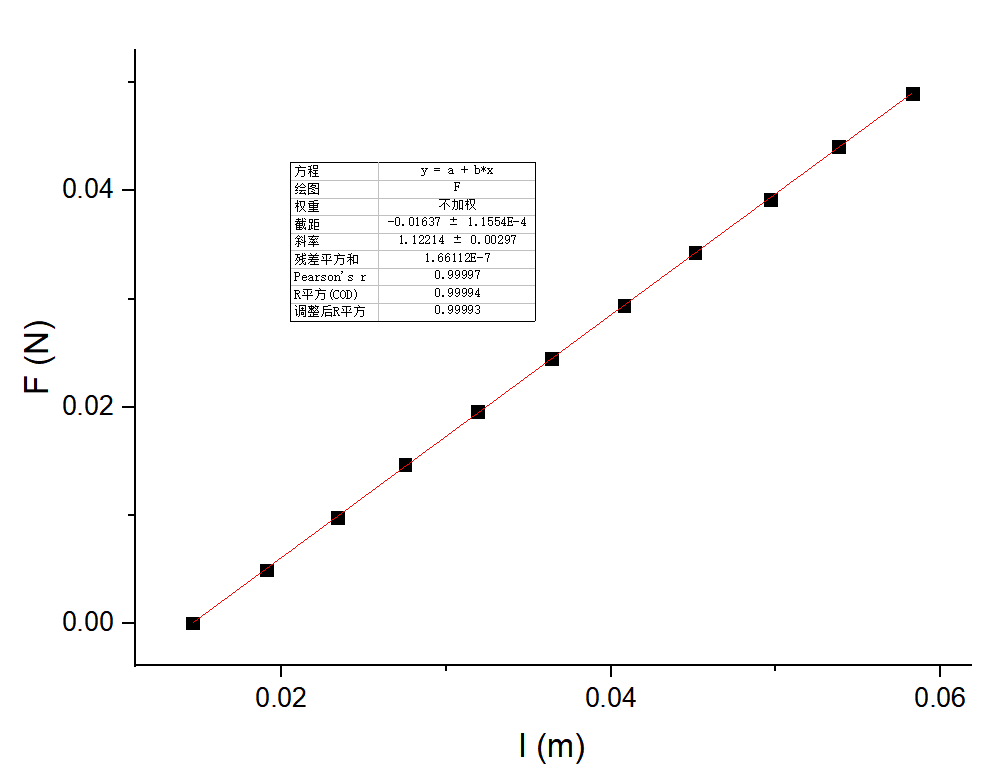
\includegraphics[scale=0.6]{11}
\\图2:弹簧劲度系数线性拟合图\\
得到$ k=1.122 N/m $\\
$ U_k=0.003 N/m ,P=0.95 $\\
金属圈直径:$ \bar{d}=\dfrac{0.0320+0.0319+0.0316}{3}=0.0318 m $\\
$ \sigma_{d}=\sqrt{\dfrac{\sum_{i=1}^{3}(d_i-\bar{d})^2}{3-1}}=0.0002 m $\\
$ \Delta_B=0.00015m $\\
$ U_{d}=\sqrt{(t_{0.95}\frac{\sigma_{d}}{\sqrt{n}})^2+(k_p\frac{\Delta_B}{C})^2}=\sqrt{(4.30\times0.0002/\sqrt{3})^2+(1.96\times0.00015/3)^2}m=0.0005m,P=0.95 $\\
$ d=(0.0318\pm0.0005)m $\\
水表面张力系数测量弹簧伸长量:$ \bar{x}=\dfrac{0.0115+0.0118+0.0118+0.0116+0.0111}{5}=0.0116 m $\\
$ \sigma_{x}=\sqrt{\dfrac{\sum_{i=1}^{5}(x_i-\bar{x})^2}{5-1}}=0.0003m $\\
$ \Delta_B=0.00002m $\\
$ U_{x}=\sqrt{(t_{0.95}\frac{\sigma_{x}}{\sqrt{n}})^2+(k_p\frac{\Delta_B}{C})^2}=\sqrt{(2.78\times0.0003/\sqrt{5})^2+(1.645\times0.00002/\sqrt{3})^2}m=0.0004m,P=0.95 $\\
$ \sigma=\frac{kx}{2\pi d}=0.065 N/m $\\
$ U_{\sigma}/\sigma=\sqrt{(\frac{U_k}{k})^2+(\frac{U_x}{x})^2+(\frac{U_d}{d})^2}=0.04 $\\
$ \sigma=(0.065\pm0.002)N/m $\\ \\
金属丝两脚距离:
:$ \bar{s}=\dfrac{0.0460+0.0459+0.0462}{3}=0.0460 m $\\
$ \sigma_{s}=\sqrt{\dfrac{\sum_{i=1}^{3}(d_i-\bar{d})^2}{3-1}}=0.00015 m $\\
$ \Delta_B=0.00015m $\\
$ U_{s}=\sqrt{(t_{0.95}\frac{\sigma_{s}}{\sqrt{n}})^2+(k_p\frac{\Delta_B}{C})^2}=\sqrt{(4.30\times0.00015/\sqrt{3})^2+(1.96\times0.00015/3)^2}m=0.0004m,P=0.95 $\\ 
洗洁精溶液:
	$ \bar{x}=\dfrac{0.0027+0.0028+0.0027+0.0028+0.0027}{5}=0.00274 m $\\
	$ \sigma_{x}=\sqrt{\dfrac{\sum_{i=1}^{5}(x_i-\bar{x})^2}{5-1}}=0.00005m $\\
	$ \Delta_B=0.00002m $\\
	$ U_{x}=\sqrt{(t_{0.95}\frac{\sigma_{x}}{\sqrt{n}})^2+(k_p\frac{\Delta_B}{C})^2}=\sqrt{(2.78\times0.00005/\sqrt{5})^2+(1.645\times0.00002/\sqrt{3})^2}m=0.00007m,P=0.95 $\\
	$ \sigma=\frac{kx}{2s}=0.0334 N/m $\\
	$ U_{\sigma}/\sigma=\sqrt{(\frac{U_k}{k})^2+(\frac{U_x}{x})^2+(\frac{U_s}{s})^2}=0.03 $\\
	$ \sigma=(0.0334\pm0.0009)N/m $\\ \\
	自配溶液:$ \sigma_1=kx/2s=1.122\time0.0037/(2\times0.0460)=0.045 N/m $\\
	$ \sigma_2=kx/2s=1.122\times0.0027/(2\times0.0460)=0.033 N/m $\\
	$ \sigma_1=kx/2s=1.122\times0.0027/(2\times0.0460)=0.033 N/m $\\
	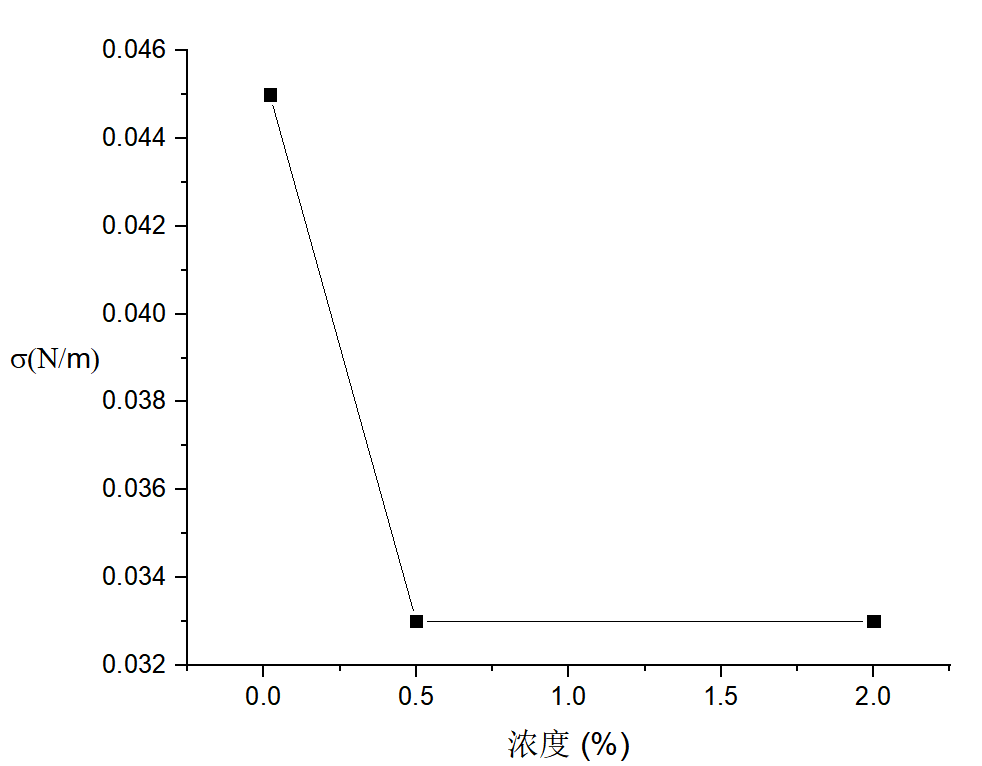
\includegraphics[scale=0.5]{12}\\
	图3:自配洗洁精溶液表面张力系数随浓度变化
	\section{实验讨论}
由实验可得,当水中加入洗洁精后,表面张力系数会减小,且随浓度增大,先迅速减小,在几乎不变。在实验时要注意使装置保持稳定,否则有震动会使液膜提前破裂,产生误差。
	\section{思考题}
1.用秤量仪器直接测量液体的表面张力,测量方法直观,概念清楚;焦利氏秤的弹簧劲度系数较小,且利用游标卡尺形式的读数方式,测量结果更加精确;实验原理简明,仪器操作简便。\\
2.正常圆柱形弹簧在越靠近上顶点处受到下方弹簧重力带来的拉力越大,导致各点的伸长量不均匀。锥形弹簧保证了弹簧在自由悬挂状态下各点的伸长量一致,抵消了重力对弹簧劲度系数的影响。\\
3.由于实验装置不够平稳,存在震荡,导致液膜提前破裂,测得表面张力系数偏小;吊环在实验时不完全水平;多次实验过程中有残存在吊环上的水的重力;面镜非完全铅垂导致与玻璃管间存在摩擦;弹簧未完全稳定即读数。
	
\end{document}